\documentclass{article}

% Packages (optional, but useful)
\usepackage[utf8]{inputenc} % Allows UTF-8 characters
\usepackage{graphicx} % Allows including images
\usepackage{listings} % Include this in the preamble
\usepackage{amsmath} % Include this in the preamble

\title{Neural Network Simplified Mathematics}
\author{Cole Gulino}
\date{\today} % Automatically insert today's date

\begin{document}

\maketitle % Generates the title, author, and date

\section{Introduction}
To improve on my deep learning fundamentals, I wanted to understand how backpropogation worked for 
most of the fundamental building blocks of neural networks (i.e. convolution, attention, etc.) Here 
I will document the results for others who are studying as well.

\section{Layers}
This file lays out the interface to all of the other modules
that will be presented in the rest of the neural network layers.

This has two main functions which should be understandable to all of users of popular languages like 
Pytorch and Jax.

\paragraph*{Forward}

\begin{lstlisting}[language=Python]
def forward(
    self, x: np.ndarray
) -> tuple[np.ndarray, Cache]:
    ...
\end{lstlisting}

\paragraph*{Backward}

In the forward pass, we assume one input although `*args` and 
`**kwargs` can be passed in. The output is a tuple of the output 
tensor (assumed single) and a `Cache` object which is a dictionary 
that will be passed into the `backward` pass.

\begin{lstlisting}[language=Python]
    backwards_gradient = din = [din_1, din_2]
\end{lstlisting}    

$$
y_1 = f_1(x)
$$
$$
y_2 = f_2(y_1)
$$
$$
y_3 = f_3(y_2)
$$

If we want to find the partial derivative $\partial y_3 / \partial 
x$, we can use the to find the derivatives.

$$
\frac{\partial y_3}{\partial x} =
\frac{\partial y_3}{\partial y_2}
\frac{\partial y_2}{\partial y_1}
\frac{\partial y_1}{\partial x}
$$

$$
f_2: din = \frac{\partial y_3}{\partial y_2}
$$
$$
f_3: din = \frac{\partial y_3}{\partial y_2}
\frac{\partial y_2}{\partial y_1}
$$

For all of our backwards gradients, we assume that the first layer is some loss function that returns a scalar, so that the the first node in the backwards graph always returns:
$$
\frac{\partial L}{\partial Y}
$$
Because $L$ is a scalar, the quantity $\partial L / \partial Y$ is a matrix of the same shape as $Y$.

For example, if we imagine that the matrix $Y$ is of shape `[M=2, C=2]` then we can write the expression as:
$$
\frac{\partial L}{\partial Y} = \begin{bmatrix}
 \frac{\partial L}{\partial y_{11}} && \frac{\partial L}{y_{12}} \\
 \frac{\partial L}{\partial y_{21}} && \frac{\partial L}{y_{22}}
\end{bmatrix}
$$ 

All of the quantities calculated will be based on this, for example $\partial L / \partial W$. Some of the intermediate quantities will be Jacobians (i.e. matrices with matrix derivatives) but we can avoid this with some tricks as will illustrate in other parts of the documentation.

\paragraph*{Other Interfaces}

These two functions make up the bulk of the functionality of the `Layer` class. The thing to call out is the `Cache` dataclass `Cache = dict[str, np.ndarray]` which is the way we cache out information for the backwards pass.

\begin{lstlisting}[language=Python]
    def update_parameters(
        self, parameters: dict[str, np.ndarray]
    ) -> None:
\end{lstlisting}

\subsection*{Attention}

The attention mechanism is the underpinning of all transformer networks as 
it calculates the attention each new token places on all of the other tokens
in the sequence. In this way it determines how each token aggregates 
information for the other tokens in the sequence. The module is rather
simple but has some interesting components for the calculation. Namely it uses
the $\textbf{softmax}$ function from above.

\paragraph*{Forward} The forward pass is rather simple and we'll lay out
a simplified version here.

We have three different quantities that the attention mechanism calculates:
$\textbf{queries}$, $\textbf{keys}$, $\textbf{values}$ which correspond to
different values in the attention computation. Queries are request information
from the other elements in the sequence. The queries are what correspond to
the output of the attention mechanism. The attention represents a weighting
of how much the queries should pay attention to each element in the sequence
and then it is used to compute a weighted sum of the $\textbf{values}$.

$$
A = \text{Softmax}\left(Q K^T / \text{scale}\right)
$$

Where $\text{scale} = 1 / \sqrt{d_{in}}$. In a similar reasoning to initialization
this scale factor ensures that the variance inside and outside of the softmax
is the same.

After the attention computation, we can calculate the weighted sum with the
values.

$$
Y = A \cdot V
$$

Oftentimes attention is computed on a causal sequencne where $x_t$ depends
on $x_{1:t-1}$ but not on anything after. During training, we have the entire
sequence and so we need a way to mask out information from the future sequence.
Because we rely on the softmax to aggregate the tokens, we can just mask out
the attention from future tokens.

$$
K = XW_K; \space Q = XW_Q; \space V = XW_V
$$

$$
A = \text{Softmax}\left((Q K^T  \cdot M) / \text{scale}\right)
$$

Where $M$ is a causal mask of something like this for a 4 element sequence.

$$
M = \begin{bmatrix}
    1 && -\inf && -\inf && -\inf \\
    1 && 1 && -\inf && -\inf \\
    1 && 1 && 1 && -\inf \\
    1 && 1 && 1 && 1 \\
    \end{bmatrix} 
$$   

\paragraph*{Backward} Given the previous gradients we have calculated,
we have all of the tools we need to compute the gradientns for the
attention mechanism.

We need to compute gradients for the weights of all of the different
projection matrices $ W_K, W_Q, W_V$ given that we have the backwards
gradient from the loss $\partial L / \partial Y$.

First we can calcualte the gradient $\partial L / \partial W_V$ which is
a matrix the same shape as $W_V$:

$$
\frac{\partial L}{\partial W_V} = \frac{\partial L}{\partial Y}\frac{
    \partial Y}{\partial V}\frac{\partial V}{\partial W_V}
$$

Let's first focus on the first side of the components. This is similar to 
what we saw before and so we can compute this without computing the
intermediate Jacobians.
$$
\frac{\partial L}{\partial v_i} = \sum_{i'}\sum_{j'}\frac{
    \partial L}{\partial y_{i'j'}}\frac{
        \partial y_{i'j'}}{\partial v_i}
$$

What we saw from the dense computation is that this corresponds to:
$$
\frac{\partial L}{\partial V} = A\frac{\partial L}{\partial Y}
$$

This becomes the backwards gradient we pass into the Dense layer $V = XW_V$.
And since we also know that computation, we can find that:
$$
\frac{\partial L}{\partial W_V} = X^T\frac{\partial L}{\partial V} =
X^TA\frac{\partial L}{\partial Y}
$$

To compute the next compoenents of the gradient, we need to backprop through
the softmax computation.
$$
\frac{\partial L}{\partial W_Q} = \frac{\partial L}{\partial Y}
\frac{\partial Y}{\partial A}\frac{\partial A}{\partial Q}
\frac{\partial Q}{\partial W_Q}
$$
$$
\frac{\partial L}{\partial W_K} = \frac{\partial L}{\partial Y}
\frac{\partial Y}{\partial A}\frac{\partial A}{\partial K}
\frac{\partial K}{\partial W_K}
$$

We immediately see that the first element of both is the backwards gradient
that we have computed before. And the second component of both is shared so
we can start with that.

$$
\frac{\partial L}{\partial A} = \frac{\partial L}{\partial Y}
\frac{\partial Y}{\partial A} = \frac{\partial L}{\partial Y}V^T
$$

This becomes the backwars gradient into the softmax computation. Which we
can recall that is is in fact a Jacobian of shape $d_{in} x d_{in}$:

Lets assume we want to break this down further so that we can rename the
input to the softmax as $Z = QK^T / scale$.

$$
\frac{\partial \text{softmax}(z_i)}{\partial z_j}
$$
if $i == j$:

$$
\frac{\partial \text{softmax}(z_i)}{\partial z_j} =
\text{softmax}(z_i)\left[1 - \text{softmax}(z_i)\right]
$$

if $i \ne j$
$$
\frac{\partial \text{softmax}(z_i)}{\partial z_j} = -
\text{softmax}(z_i)\text{softmax}(z_j)
$$

And first we can find the derivative with respect to $Z$.
$$
\frac{\partial L}{\partial Z} = \frac{\partial L}{\partial Y}
\frac{\partial Y}{\partial A}\frac{\partial A}{\partial Z}
$$

The softmax operator works on a vector and not a matrix. You know this
because you are required to provide a $\text{dim}$ parameter to the 
softmax function to know which vector it operates on.

Imagine $Z$ is a square matrix (as it will be):
$$
Z = \begin{bmatrix}
    z_{11} && z_{12} \\ z_{21} && z_{22}
\end{bmatrix}
$$

And that we will be operating along the column dimension so that we
get the derivatives with respect to some row.

$$
Z = \begin{bmatrix}
    Z_1 \\ Z_2
\end{bmatrix}
$$

So we can look at this from a row level and say we can calculate the
derivatives w.r.t. each row and then combine them i.e. 
$\partial A_i / \partial Z_i$.

So for example row 1:
$$
\frac{\partial L}{\partial Z_1} =
\frac{\partial L}{\partial A_1}
\frac{\partial A_1}{Z_1}
$$

$$
\frac{\partial L}{A_1} = \begin{bmatrix}
    \partial L / \partial a_{11} && \partial L / \partial a_{12}
\end{bmatrix}
$$

This quantity is a vector derivative w.r.t. another vector and so we have
a Jacobian of shape $d_{A_1} x d_{Z_1}$

$$
\frac{\partial A_1}{\partial Z_1} = \begin{bmatrix}
    \partial a_{11} / \partial z_{11} && \partial a_{12} \partial z_{11} \\
    \partial a_{11} / \partial z_{12} && \partial a_{12} \partial z_{12}
\end{bmatrix}
$$

From the definition of the softmax derivative we can find:
$$
\frac{\partial A_1}{\partial Z_1} = \begin{bmatrix}
    a_{11}\left[1 - a_{11}\right] && 
    -a_{12}a_{11} \\
    -a_{11}a_{a_{12}} && 
    a_{12}\left[1 - a_{12}\right]
\end{bmatrix}
$$

$$
\frac{\partial L}{\partial Z_1} =
\begin{bmatrix}
    \partial L / \partial a_{11} && 
    \partial L / \partial a_{12}
\end{bmatrix}
\begin{bmatrix}
    a_{11}\left[1 - a_{11}\right] && 
    -a_{12}a_{11} \\
    -a_{11}a_{a_{12}} && 
    a_{12}\left[1 - a_{12}\right]
\end{bmatrix}
$$
$$
\frac{\partial L}{\partial Z_1} =
\begin{bmatrix}
    \frac{\partial L}{\partial a_{11}}a_{11}(1 - a_{11}) -
    \frac{\partial L}{\partial a_{12}}a_{11}a_{12} &&
    -\frac{\partial L}{\partial a_{11}}a_{11}a_{12} +
    \frac{\partial L}{\partial a_{12}}a_{12}(1 - a_{12})
\end{bmatrix}
$$

We can do this same thing for other rows to get the final calculation.
$$
\frac{\partial L}{\partial Z} =
\begin{bmatrix}
    \frac{\partial L}{\partial a_{11}}a_{11}(1 - a_{11}) -
    \frac{\partial L}{\partial a_{12}}a_{11}a_{12} &&
    -\frac{\partial L}{\partial a_{11}}a_{11}a_{12} +
    \frac{\partial L}{\partial a_{12}}a_{12}(1 - a_{12}) \\

    \frac{\partial L}{\partial a_{21}}a_{21}(1 - a_{21}) -
    \frac{\partial L}{\partial a_{22}}a_{21}a_{22} &&
    -\frac{\partial L}{\partial a_{21}}a_{21}a_{22} +
    \frac{\partial L}{\partial a_{22}}a_{22}(1 - a_{22})
\end{bmatrix}
$$

Now remember that $Z = QK^T / \text{scores}$. And now we want to find
$\partial L / \partial Q$ and $\partial L / \partial K$. 

Since we know the derivative w.r.t. $Z$ we can just calculate:
$$
\frac{\partial L}{\partial Q} = \frac{\partial L}{\partial Z}
\frac{\partial Z}{\partial Q}; \space
\frac{\partial L}{\partial K} = \frac{\partial L}{\partial Z}
\frac{\partial Z}{\partial K}
$$
We know that:
$$
Z =  \begin{bmatrix}
    q_{11} & q_{12} \\ q_{21} & q_{22}
\end{bmatrix}  \begin{bmatrix}
    k_{11} & k_{21} \\ k_{12} & k_{22}
\end{bmatrix}= \begin{bmatrix}
    q_{11}k_{11} + q_{12}k_{12} & q_{11}k_{21} + q_{12}k_{22} \\
    q_{21}k_{11} + q_{22}k_{12} & q_{21}k_{21} + q_{22}k_{22}
\end{bmatrix}
$$

So for K:
$$
\frac{\partial L}{\partial k_{ij}} = 
\sum_{i'}\sum_{j'}\frac{\partial L}{\partial z_{i'j'}}
\frac{\partial z_{i'j'}}{\partial k_{ij}}
$$

$$
\frac{\partial Z}{\partial k_{11}} = \begin{bmatrix}
   q_{11} & 0 \\ q_{21} & 0
\end{bmatrix}; \space 
\frac{\partial Z}{\partial k_{12}} = \begin{bmatrix}
    q_{12} & 0 \\ q_{22} & 0
\end{bmatrix}
$$
$$
\frac{\partial Z}{\partial k_{21}} = \begin{bmatrix}
    0 & q_{11} \\ 0 & q_{21}
\end{bmatrix}; \space 
\frac{\partial Z}{\partial k_{22}} = \begin{bmatrix}
    0 & q_{12} \\ 0 & q_{22}
\end{bmatrix}
$$

$$
\frac{\partial L}{\partial K} = \frac{\partial L}{\partial Z}^TQ
$$
And then similarly for q
$$
\frac{\partial L}{\partial Q} = \frac{\partial L}{\partial Z}^TK
$$

We can then compute the same computations for the dense layers that
connect to these to get the gradients w.r.t. the weight matrices and the
input $X$.

Because $X$ forks here into $Q, K, V$ we need to sum up the contributions
of the gradients from each.

$$
\frac{\partial L}{\partial X} = 
\frac{\partial L}{\partial Q}\frac{\partial Q}{\partial X} +
\frac{\partial L}{\partial K}\frac{\partial K}{\partial X} +
\frac{\partial L}{\partial V}\frac{\partial V}{\partial X}
$$

\subsection*{Transformer Block}

The transformer block is just a combination of many things
we've seen above including attention from above.

The simplest form of the block is easier to write in code:

\begin{lstlisting}[language=Python]

def ffn(x):
    x = mlp_1(x)
    x = relu(x)
    x = mlp_2(x)
    return x

x = x + attn(ln_attn(x))
x = x + ffn(ln_ffn(x))
\end{lstlisting}
Here we are looking at prenorm where the layer norm happens before the
functions $\text{attn}$ and $\text{ffn}$.

We have seen how we can cascade gradients as backwards from before. The 
new thing here is managing the skip connection. Here we have two, one after
the $\text{attn}$ and one after the $\text{ffn}$.

If we have a function with a residual connection:
$$
y = x + f(x)
$$

The derivative then is:
$$
\frac{\partial y}{\partial x} = \frac{\partial}{\partial x}x +
\frac{\partial}{\partial x}y(x)
$$
$$
\frac{\partial y}{\partial x} = 1 +
\frac{\partial}{\partial x}y(x)
$$

We can rewrite the code above as some functions:
$$
y_1 = x + \text{attn}\left(\text{ln}_1\left(x\right)\right)
$$
$$
y_2 = y_1 + \text{ffn}\left(\text{ln}_2\left(y_1\right)\right)
$$

Lets say $z_1 = \text{ln}_1\left(x\right)$ and 
$z_2 = \text{ln}_2\left(y_1\right)$.

$$
y_1 = x + \text{attn}\left(z_1\right)
$$
$$
y_2 = y_1 + \text{ffn}\left(z_2\right)
$$


For our gradients we want to find the output w.r.t. x:
$$
\frac{\partial y_2}{\partial x} = 
\frac{\partial y_2}{\partial y_1}
\frac{\partial y_1}{\partial z_2}
\frac{\partial z_2}{\partial y_1}
\frac{\partial y_1}{\partial z_1}
\frac{\partial z_1}{\partial x}
$$

$$
\frac{\partial y_2}{\partial y_1} = 
1 + 
\frac{\partial \text{ffn}(\text{ln}_2(y_1))}{\partial \text{ln}_2(y_1)}
\frac{\partial \text{ln}_2(y_1)}{\partial y_1}
$$

When we know that the backwards gradient exists 
$\partial L / \partial y_2$.

$$
\frac{\partial L}{\partial y_1} = 
\frac{\partial L}{\partial y_2} + 
\frac{\partial L}{\partial y_2}
\frac{\partial \text{ffn}(\text{ln}_2(y_1))}{\partial \text{ln}_2(y_1)}
\frac{\partial \text{ln}_2(y_1)}{\partial y_1}
$$

From this we can see that the first term is the skip connection 
contribution and the second term is the backwards gradients from all of
the different layers to get to $y_1$.

$$
\frac{\partial y_1}{\partial x} = 
1 + 
\frac{\partial \text{attn}(\text{ln}_1(x))}{\partial \text{ln}_1(x)}
\frac{\partial \text{ln}_1(x)}{\partial x}
$$

$$
\frac{\partial L}{\partial x} = 
\frac{\partial L}{\partial y_1} + 
\frac{\partial L}{\partial y_1}
\frac{\partial \text{attn}(\text{ln}_1(x))}{\partial \text{ln}_1(x)}
\frac{\partial \text{ln}_1(x)}{\partial x}
$$

$$
\frac{\partial L}{x} = 
\frac{\partial L}{\partial y_2} +
\frac{\partial L}{\partial y_2}
\frac{\partial \text{ffn}(\ln_2(y_1))}{\partial \ln_2(y_1)}
\frac{\partial \ln_2{y_1}}{\partial y_1} +
\frac{\partial L}{\partial y_1}
\frac{\partial \text{attn}(\ln_1(x))}{\partial \ln_1(x)}
\frac{\partial \ln_1(x)}{\partial x}
$$

This in code looks like:

\begin{lstlisting}[language=Python]
backwards_gradient = (
    backwards_gradient +
    backwards_gradient_ln_1 +
    backwards_gradient_ln_2
)
\end{lstlisting}

\section*{Optimization}

\subsection*{Optimizers}
\subsubsection*{Stochastic Gradient Descent}

\begin{figure}[htbp]
    \centering
    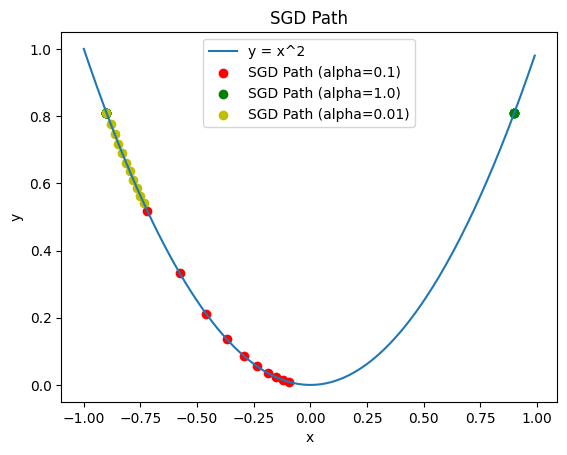
\includegraphics[width=\linewidth]{images/sgd.png}
    \caption{Stochastic gradient descent with different learning rates.}
    \label{fig:sgd}
\end{figure}

The simplest form of optimization is stocahstic gradient
descent where you take a small step in the direction
of the gradient.

$$
\theta = \theta - \alpha \nabla \theta
$$

Stochastic gradient descent is incredibly simple and can
be written in a few lines of code.

\begin{lstlisting}[language=Python]
for k in self.parameters:
\end{lstlisting}

\subsubsection*{Momentum}

Momentum is a simple adaptation to the SGD algorithm which adds
a momentum term to the update. This helps smooth out the gradients
it replaces the gardient calculation with a weighted combination 
average of previous gradients. This helps smooth out noise in the
gradient computation.

$$
\mu_{t} = \beta \mu_{t-1} + 
(1 - \beta)\nabla \theta
$$
$$
\theta = \theta - \alpha \mu_t
$$

\subsubsection*{Adam}
Adam is a very popular optimizer as it takes momentum a bit further
and calculates the second order running statistics as well. It computes
a momentum term as well.

$$
\mu = \beta_1 \mu + (1 - \beta_1)\nabla \theta
$$

It also calcualtes a standard deviation.
$$
v = \beta_2 v + (1 - \beta_2)(\nabla \theta) ^ 2
$$

It then normalizes these values before the update to ensure that
they are well behaved and averaged over the time horizon $T$.
$$
\hat \mu = \frac{\mu}{1 - \beta_1T}
$$
$$
\hat v = \frac{v}{1 - \beta_2T}
$$
The final update is given by:
$$
\theta = theta - \alpha \frac{\hat \mu}{\sqrt{\hat v}}
$$

\subsection*{Regularization and Normalization}
Optimization can be helped a number of ways including 
regularizing the network and normalization after different
layers. Regularization limits the capacity of the network
and normalization better conditions the activations.

\subsubsection*{Dropout}
Dropout is one of the most widely used regularization 
techniques and is very simple.

A mask is sampled randomly of zeros and ones. This mask is
then applied to the input of the function.

\begin{lstlisting}[language=Python]
def dropout_forward(x, p):
    mask = (np.random.random(x.shape) > p).astype(float)
    return x * mask
\end{lstlisting}    

The backwards pass is just as simple.
\begin{lstlisting}[language=Python]
def dropout_backward(mask, dout):
    return dout * mask
\end{lstlisting}    

\subsubsection*{Layer Norm}

LayerNorm is a popular normalization scheme and has recently
become one of the go to normalization components for the popular
transformer networks. 

Other normalization schemes like BatchNorm keep running statistics
of the values of each batch. This allows it to normalize the
layers as a running average over the entire dataset. While this
may be appealing, it has some downsides. It's very computationally
and memory inefficient (especially when it has to sync over
multi-GPU training). LayerNorm gets around that by normalizing each
activation separately and centered to the activation itself and not
to the dataset statistics.

\paragraph*{Forward}For each element in the batch we compute these statistics:
$$
\mu = \frac{1}{D}\sum_{d=1}^D x_d
$$
$$
\sigma^2 = \frac{1}{D}\sum_{d=1}^D(x_d - \mu)^2
$$

And with this we can normalize our values.
$$
\hat x = \frac{x - \mu}{\sigma^2}
$$

The layer also has some small learnable parameters the same
shape as the number of dimensions of the input $D$. They apply
a learned scale and shift so that the network can slightly modify
the normalization for better learning. It's customary to initialize
these to do nothing (i.e. scale to 1 and shift to 0).

$$
y = \gamma \hat x + \beta
$$

\paragraph*{Backward}
\subsection*{Losses}
\end{document}
